\section{Algorithm Compiler}\label{sec:compiler}

\begin{figure}
  \centering
  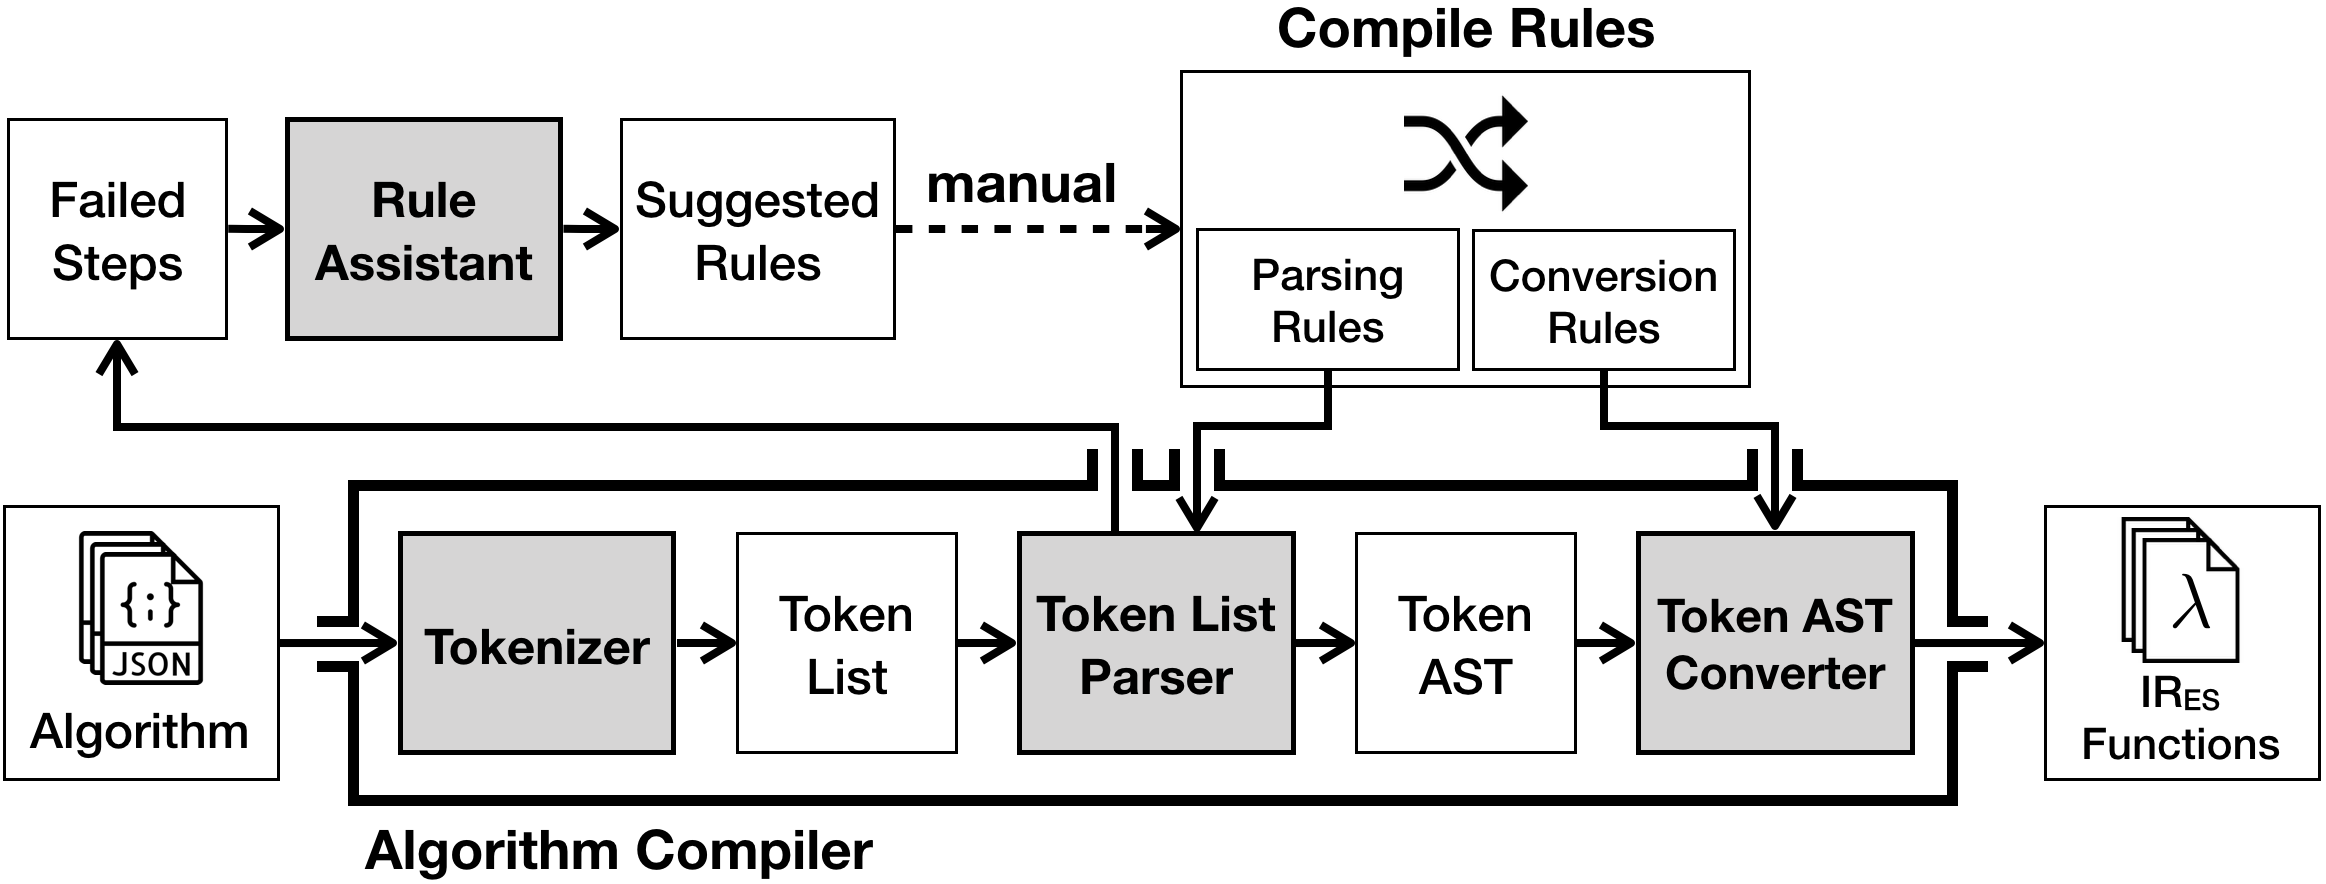
\includegraphics[width=0.5\textwidth]{img/algo_compiler.png}
  \caption{Overall structure of the algorithm compiler.}
  \label{fig:algo-compiler}
\end{figure}

In this section, we propose the \textit{algorithm compiler}
that compiles abstract algorithms into \( \ires \) functions
and its overall structure is described in Figure~\ref{fig:algo-compiler}.
Before compiling abstract algorithms,
the tokenizer first tokenizes each abstract algorithm into
a list of tagged tokens. Then, the token parser constructs
abstract syntax tree (AST) of the given token list.
Finally, the \( \ires \) matcher constructs the corresponding
\( \ires \) function from the given token AST.
The parser and the matcher are dependent on compile rules
and we define the general compile rules for abstract algorithms in
ECMAScript specifications. Like Coq, a proof assistant, we also provide
the \textit{rule assistant} to make easy write compile rules.
It suggests new compile rules based on
statistical analysis of failed algorithm steps to be parsed
and also diagnoses root causes of parsing failures
for updated abstract algorithms.

\subsection{Tokenizer}

Abstract algorithms in ECMAScript specifications are written in structured
natural languages in HTML files. An algorithm consists of ordered steps
and it might contain sub-steps as well. For example,
the ToPrimitive algorithm in Figure~\ref{fig:to-primitive-es}
has three steps and second step has seven sub-steps.
Moreover, the tokens of each step has its own HTML tag and each tag
has the following meaning:
\[
  \begin{array}{c|l}
    \text{HTML tags} & \text{meanings}\\\hline\hline
    \code{<var>} & \text{variables}\\\hline
    \code{<emu-grammar>} & \text{productions}\\\hline
    \code{<emu-nt>} & \text{non-terminal syntax}\\\hline
    \code{<code>} & \text{ECMAScript codes}\\\hline
    \code{<emu-const>} & \text{constant values}\\\hline
    \code{<emu-val>} & \text{values}\\\hline
    \code{<ol>} & \text{ordered sub-steps}\\\hline
    \code{<ul>} & \text{unordered sub-steps}\\\hline
    \code{<sup>} & \text{superscripts}\\\hline
    \text{otherwise} & \text{simple texts}\\\hline
  \end{array}
\]
We try to keep the tag information for each token to generate more
precise compile rules. For example, if and only if a token has a tag
\( \code{<var>} \), it is a parameter or a local variable.
Thus, it is possible to construct a compile rule precisely discriminates
identifiers and other components.

The tokenizer first recognizes the overall structures of steps.
Then, it divides each step into sequence of tagged tokens.
If an HTML element has a explicit tag, it is converted into a single token
with the tag. Otherwise, it is divided into multiple tokens and each token
should be a sequence of alphanumeric characters or a single
non-alphanumeric character. For example, in the ToPrimitive algorithm,
\( \textbf{\code{"default"}} \) is a single token with the HTML tag \( \code{<code>} \)
and \( \code{@@toPrimitive} \) is divided into three text tokens
\( \code{@} \), \( \code{@} \), and \( \code{toPrimitive} \).

Moreover, the tokenizer flattens the structured steps into
a single token list to easily handle multi-step statements.
Several statements in abstract algorithms consists of multilple steps.
For example, an if-then-else statement often consists of two steps;
one step for the then-branch and another step for the else-branh.
For linear structures, we introduce three special tokens to break down structured
algorithms; \( \tend \) denotes the end of a single step,
\( \tin \) and \( \tout \) the start and the end of nested steps, respectively.
For example, the ToPrimitive algorithm is tokenized as follows.
\[
  \begin{array}{l}
    \code{Assert} \cdots \tend\\
    \code{If} \cdots \tin \code{If} \cdots \tend
    \cdots \code{Return} \cdots \tend \tout \tend\\
    \code{Return} \cdots \tend\\
  \end{array}
\]

After tokenizing abstract algorithms, the algorithm compiler compiles token lists
into \( \ires \) functions. It consists of two modules; the token list parser and
the token AST converter. They are dependent on compile rules and each compile rule
consists of a \textit{parsing rule} and a \textit{conversion rule}:
\begin{lstlisting}[style=myScalastyle]
val CompileRule = ParsingRule ^^ ConversionRule
\end{lstlisting}
For the compile rule \( \code{CompileRule} \), the parsing rule
\( \code{ParsingRule} \) describes how to parse the given token list into structured
token AST. The conversion rule \( \code{ConversionRule} \) describes how to
convert the given token AST structure into an \( \ires \) component.
Now, we explain the token list parser and token AST converter with
parsing rules and conversion rules, respectively.

\subsection{Token List Parser}

The token list parser is dependent on the given parsing rules.
Each parsing rule is written in extended Scala parser combinators.
We modify the meaning of alternative composition operator ( \( | \) ) to collect
all longest matched results. If the parser detects that a step cannot be
parsed with the given parsing rules. It reports that the step is not possible
to be parsed under the given rules into the rule assistant.
Moreover, even though the parser could parse the step, it will be also reported
if it could be parsed in not a single but multiple ways.
We basically use Packrat parsing~\cite{packrat}, the parsing rule could support
not only non-left recursive but also left recursive parsing rules.

We support two kinds of basic token parsers; tag-based parsers and
content-based parsers. A tag-based parser just checks that the next
token has the given tag. For example, the tag-based parser \( \code{varT} \)
checks that the next token has the tag \( \code{<var>} \). A content-based parser
checks that the next token is text token and its content passes the given condition.
For example, the String literal \( \code{"Let"} \) denotes the content parser
that checks whether the next token is text token with the content \( \code{Let} \).
Moreover, we provide two content parsers \( \code{word} \) and \( \code{number} \)
that checks the content consists of only alphabets or numbers, respectively.
In the parsing rule, any helper functions defined in Scala parser combinators
are available. For example, the helper function \( \code{repsep(p, q)} \) generates a new
parsing rule that denotes zero or more repetitions of the parsing rule \( \code{p} \)
using another parsing rule \( \code{q} \) as the separator.

For example, the following parsing rule is simplified version for
the step 2-e-i of the ToPrimitive algorithm.
\begin{lstlisting}[style=myScalastyle]
// statements
val Stmt = "Let" ~ varT ~ "be" ~ Expr ~ "." ^^ ...
// expressions
val Expr = (
  // identifiers
  varT ^^ ... |
  // return if abrupt
  "?" ~ Expr ^^ ... |
  // function calls
  word ~ "(" ~ repsep(Expr, ",") ~ ")" ^^ ... |
  // lists
  "<<" ~ repsep(varT, ",") ~ ">>" ^^ ...
)
\end{lstlisting}
The \( \code{Stmt} \) denotes the compile rule for statements with one
parsing rule. The \( \code{Expr} \) represents the compile rule for expressions
with four different parsing rules. Finally, the token parser with the above rules
parses the step 2-e-i in the ToPrimitive into the following
token AST:
\begin{center}
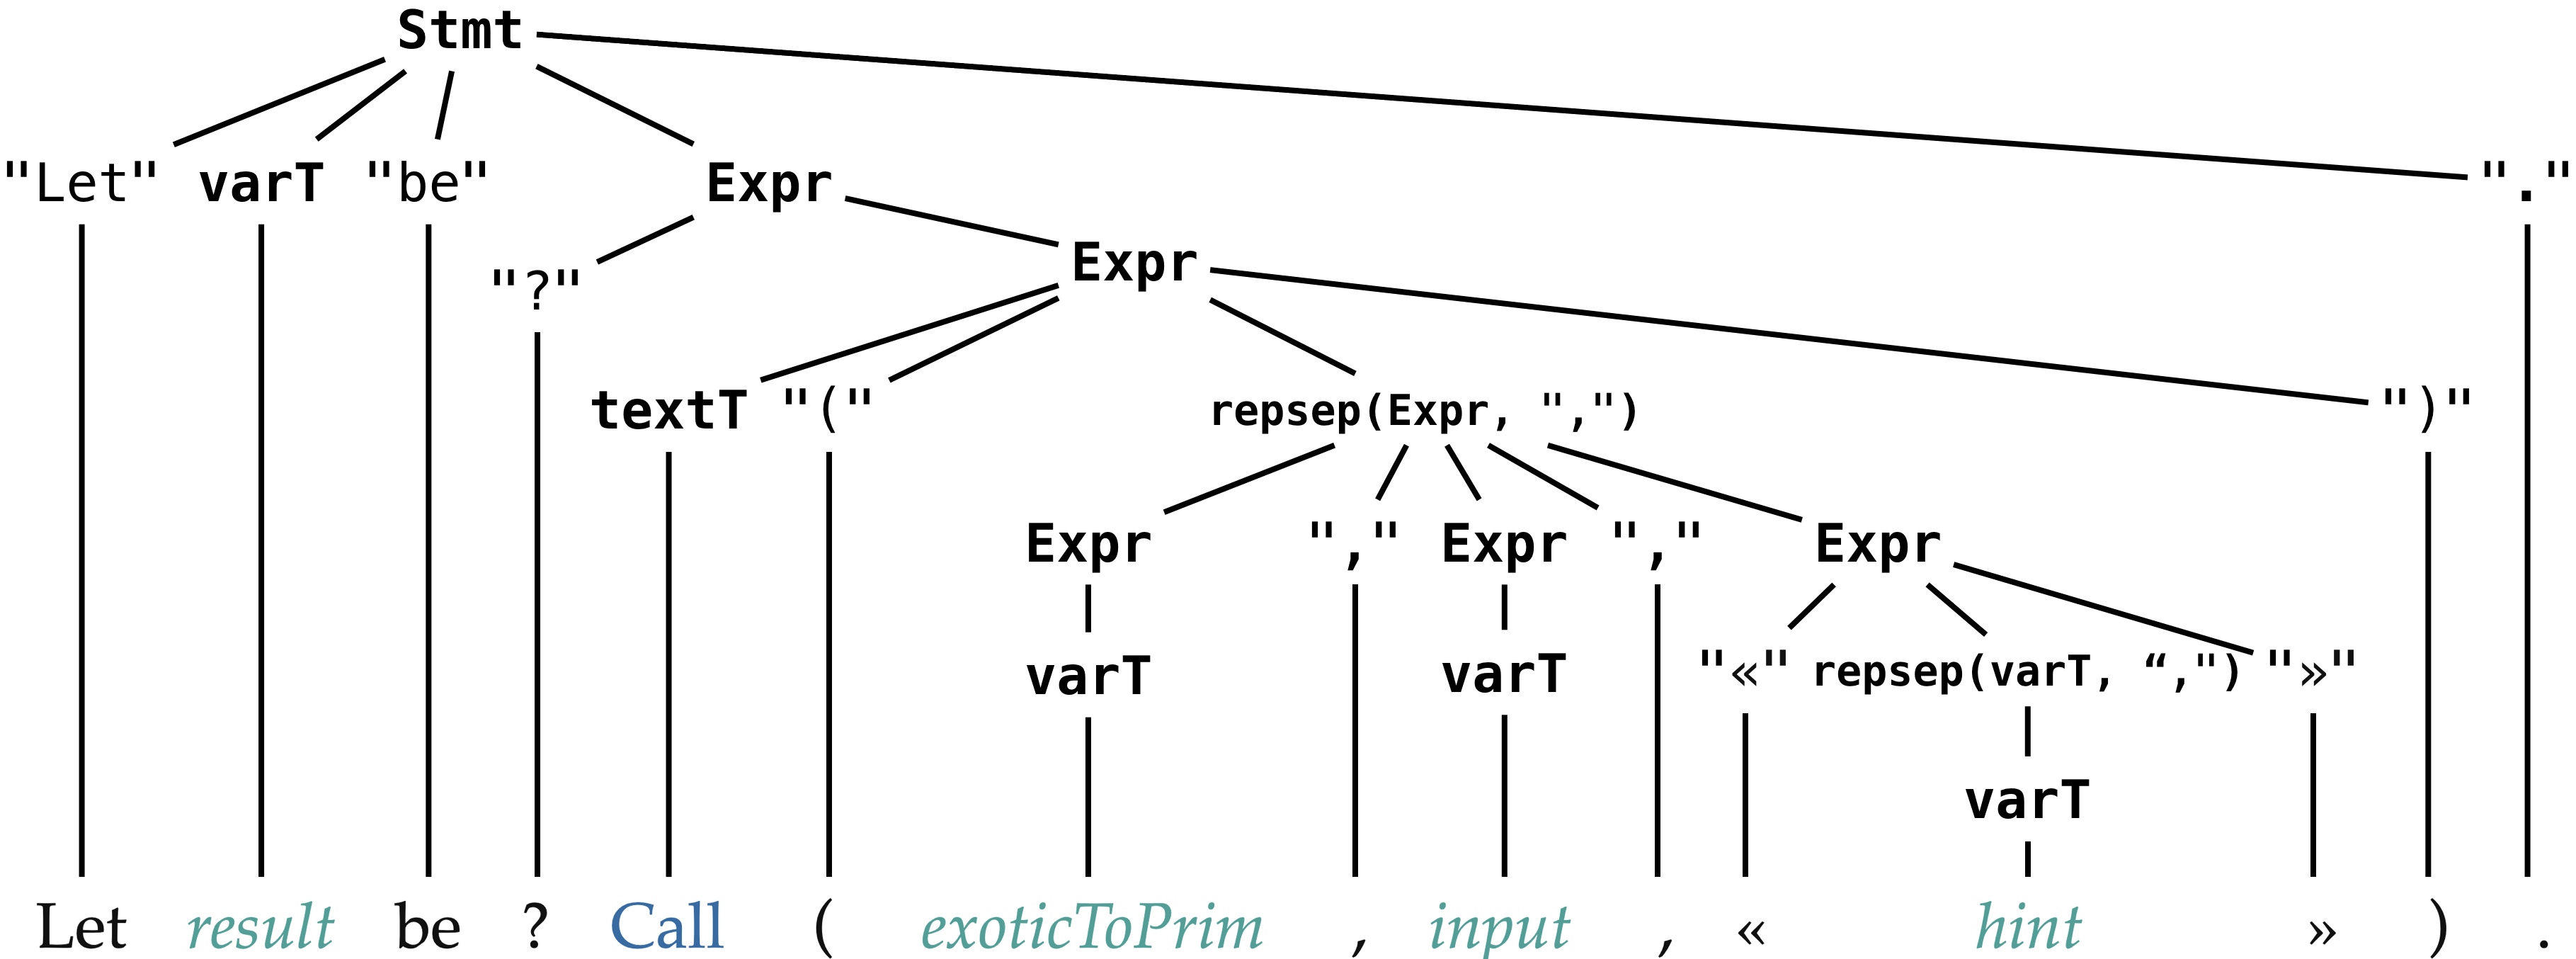
\includegraphics[width=0.5\textwidth]{img/token_ast.png}
\end{center}

\subsection{Token AST Converter}

We define \( \ires \) to represent abstract algorithms as its functions.
The following bullets explain the reason of our language design choices
for \( \ires \).

\begin{itemize}
\item \textbf{Dynamic Typing} We decide to use dynamic typing for \( \ires \)
because each variable in abstract algorithms are not statically typed.
Thus, variables do not have its own static types while each value of \( \ires \)
has its dynamic type.

\item \textbf{Imperative Style} \( \ires \) represents algorithm steps
as imperative-style instructions. Each instruction changes the current state
that consists of an environment and a heap.

\item \textbf{Higher-order Functions with Restricted Scopes} \( \ires \) supports
lambda functions as values but they have only restricted scopes. In each function,
only global variables, parameters, and newly defined local variables are available.
It means that the function closure does not capture the current environment.
We use such restricted scopes because it is enough to represent abstract algorithms.

\item \textbf{Primitive Values} \( \ires \) supports ECMAScript primitive values except
the symbols that is newly introduced after ECMAScript 6. In JavaScript, symbols are
primitive values but it is much easier to treat them as singleton objects.
Thus, only five ECMAScript primitives are defined in \( \ires \);
numbers, strings, booleans, \( \code{undefined} \), and \( \code{null} \).
Moreover, \( \ires \) also supports the unique \( \code{absent} \) value to represent
the absence of parameters. For example, the second parameter \( \code{PreferredType} \)
of ToPrimitive algorithm in Figure~\ref{fig:to-primitive-es} might be
not present in some function calls. Then, the parameter has the \( \code{absent} \) value
to represent its absence.

\item \textbf{Abstract Data Types} \( \ires \) only supports three abstract data types;
\( \code{Record} \) for mapping from some values into other value,
\( \code{List} \) for sequential data types,
and \( \code{Singleton} \) for singleton data types.
They are stored in corresponding addresses in the heap structure.
For example, ECMAScript environment records are represented as \( \code{Record} \) data types
String values as keys and addresses as values. Each key String value represents an identifier
name and each address represents an ECMAScript binding object.
Thus, the addresses point to other \( \code{Record} \) data types that represent ECMAScript bindings
in the heap. We treat not only symbols but also constants used in ECMAScript specifications,
such as \( \code{empty} \) or \( \code{normal} \), as singleton data types in \( \ires \).
\end{itemize}

To generate the corresponding \( \ires \) function from the given token AST,
the token AST converter uses the given coversion rules. Each conversion rule is
defined with the corresponding parsing rule and it is a function from given token AST
into an \( \ires \) component. For basic token parsers, their conversion rules
always return the String value of the content in the parsed token.
For example, the following conversion rules are for the previous example
parsing rules:
\begin{lstlisting}[style=myScalastyle]
// statements
val Stmt = ... ^^ { case _ ~ x ~ _ ~ y => ILet(x, y) }
// expressions
val Expr = (
  // identifiers
  ... ^^ { x => EId(x) } |
  // return if abrupt
  ... ^^ { _ ~ e => EReturnIfAbrupt(e) } |
  // function calls
  ... ^^ { case x ~ _ ~ y ~ _ => ECall(x, y) } |
  // lists
  ... ^^ { case _ ~ x ~ _ => EList(e) }
)
\end{lstlisting}
The conversion rule of the compile rule \( \code{Stmt} \) takes
only second and fourth sub trees and convert them into \( \ires \) components.
The second sub-tree is converted into a String value because it was
constructed via basic the token parser \( \code{varT} \).
The fourth sub-tree is converted into an \( \ires \) expression
because the conversion rules of the \( \code{Expr} \) compile rule
constructs \( \ires \) expressions.
Then, the conversion rule of \( \code{Stmt} \) constructs the
lexical binding instruction \( \code{ILet} \) with the String value
and the \( \ires \) expression. Finally, sub-step 2-e-i in the ToPrimitive
is converted into the following instruction:
\begin{lstlisting}[style=ires]
let result = ? (Call exoticToPrim input (new [hint]))
\end{lstlisting}


\subsection{Rule Assistant}

To make easy write compile rules, we support \textit{rule assistant}.
It takes currently not yet convertible steps as arguments
and we call them as failed steps. For each failed step,
The rule assistant diagnosis the root cause of parsing failures.
The basic idea is to check that it becomes possible to be parsed
with assumption that a speicific sub-sequence of failed steps is
successfully parsed. We define the approach to find such sub-sequences of
failed steps as \textit{fault localizations}. The rule assistant recommend
new compile rules for failed steps via fault localizations.
Moreover, it also helps us update existing compile rules for new version
of specifications.

The fault localization algorithm is evaluated with the special token \( \tstar \).
The special token \( \tstar \) represents a sub-sequence of a failed step.
The rule assistant substitues a specific sub-sequence \( T[i..j] \) of the
failed step \( T \) into a single star token \( \tstar \). For each compile rule,
the parsing rule  \( \code{starT} \) is implicitely added to utilize it in the
rule assistant. The \( \code{starT} \) is a special basic token parser
that just checks whether the given token is the special token \( \tstar \).
Its corresponding conversion rule is a function that returns a dummy
\( \ires \) component \( \code{Dummy} \) with the String value of the
compile rule name. For example, the compile rules in the previous example are
acutally defined as follows:
\begin{lstlisting}[style=myScalastyle]
// statements
val Stmt = ... | starT ^^ { case x => Dummy("Stmt") }
// expressions
val Expr = ... | starT ^^ { case x => Dummy("Expr") }
\end{lstlisting}
Then, the rule assistant evaluates the \textsc{FaultLocalize} algorithm
with the failed step to find the set of most specific suggestions.
\begin{algorithm}
  \caption{Fault Localization}
  \begin{algorithmic}[1]
    \Function{FaultLocalize}{$T,n$}\Comment{$T$ - failed step, $n$ - size}
    \State $S = \varnothing$
    \For{$i = 0$ to $n - 1$}
    \For{$j = i$ to $n - 1$}
    \State $T'$ = a copy of $T$
    \State Substitue $T'[i..j]$ into $\tstar$
    \If{Parse($T'$) containing $\code{Dummy(}x \code{)}$}
    \State Insert $(x, i, j)$ into $S$
    \EndIf
    \EndFor
    \EndFor
    \While{$s = (x, i, j) \in S$}
    \If{$\exists (y, p, q) \in S$ s.t. $i \leq p \wedge q \leq j$}
    \State Remove $s \in S$
    \EndIf
    \EndWhile
    \State \Return $S$
    \EndFunction
  \end{algorithmic}
\end{algorithm}

For example, assume that the expression compile rule for lists is removed.
Then, the step 2-e-i of the ToPrimitive algorithm becomes a failed step.
The fault localization algorithm first find one suggestion for statements
and four suggestions for expressions as follows:
\[
  \begin{array}{c}
    (\code{"Stmt"}, 0, 14), \;
    (\code{"Expr"}, 3, 13), \;
    (\code{"Expr"}, 4, 13), \;\\
    (\code{"Expr"}, 6, 12), \;
    (\code{"Expr"}, 10, 12)
  \end{array}
\]
However, first four suggestions are removed because the last one is the most
specific sub-sequence. Finally, the rule assistant suggests to define
another expression compile rule for the token list \hint{}.
